\chapter{Задание №5}

Значение регистра `x31` на момент окончания выполнения программы равно 9, как предполагалось ранее.

\begin{figure}
    \centering
    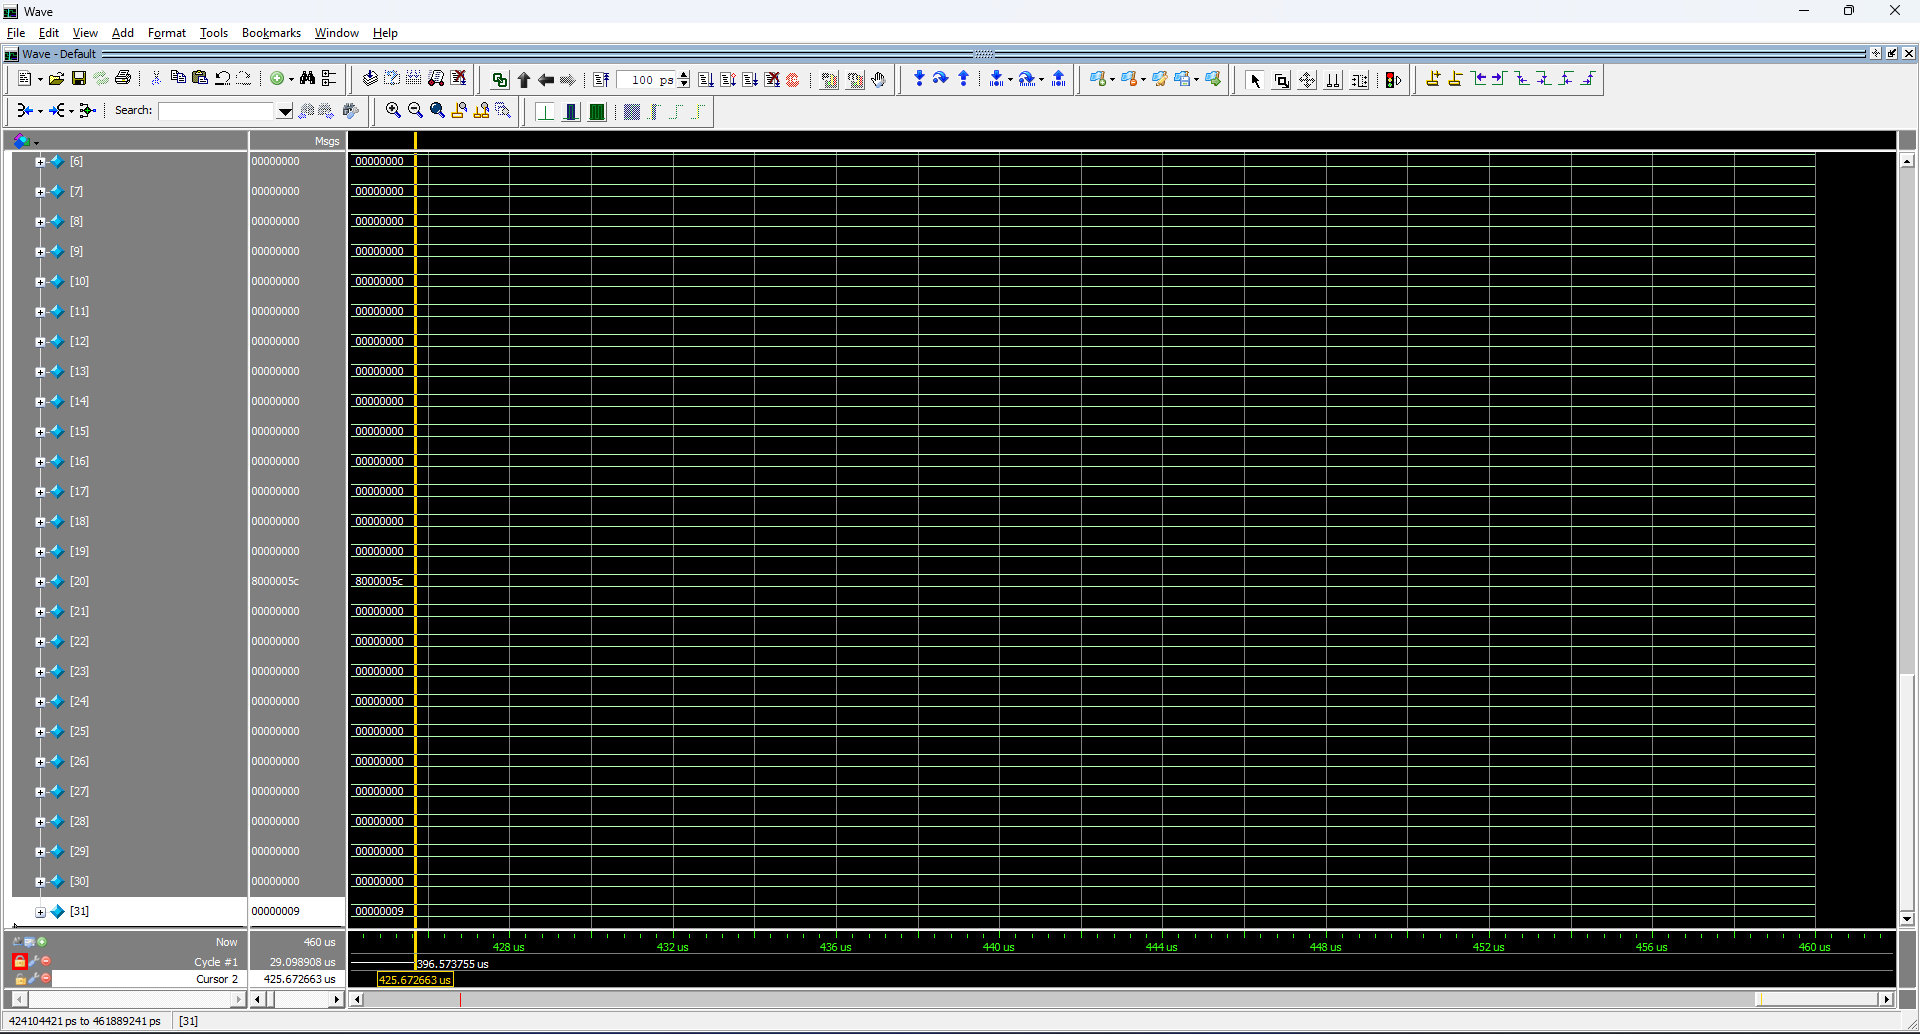
\includegraphics[width=1\linewidth]{images/05-x31_finally.png}
    \caption{Значение регистра x31 на момент окончания выполнения программы}
    \label{fig:05-x31_finally}
\end{figure}

\begin{figure}
    \centering
    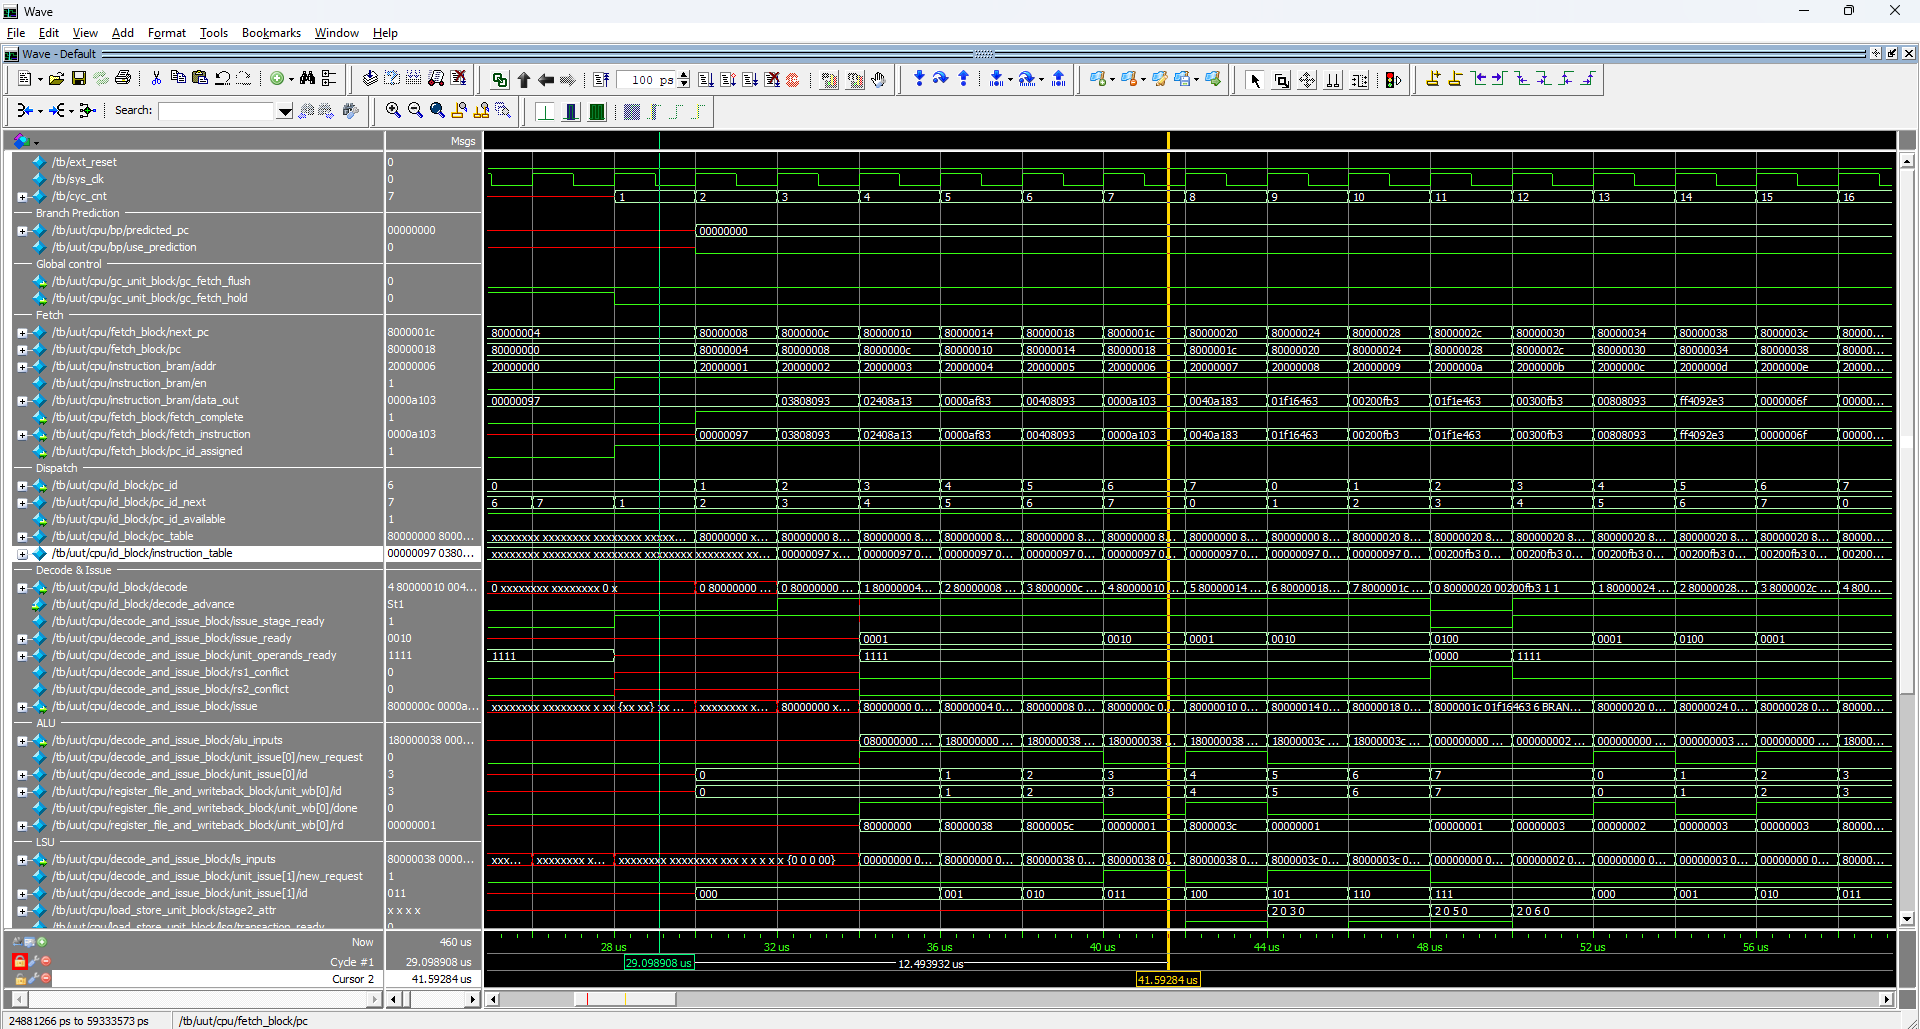
\includegraphics[width=1\linewidth]{images/05-fetch.png}
    \caption{Временная диаграмма сигналов команды lw x3, 4(x1) на стадии выборки и диспетчеризации}
    \label{fig:05-fetch}
\end{figure}

\begin{figure}
    \centering
    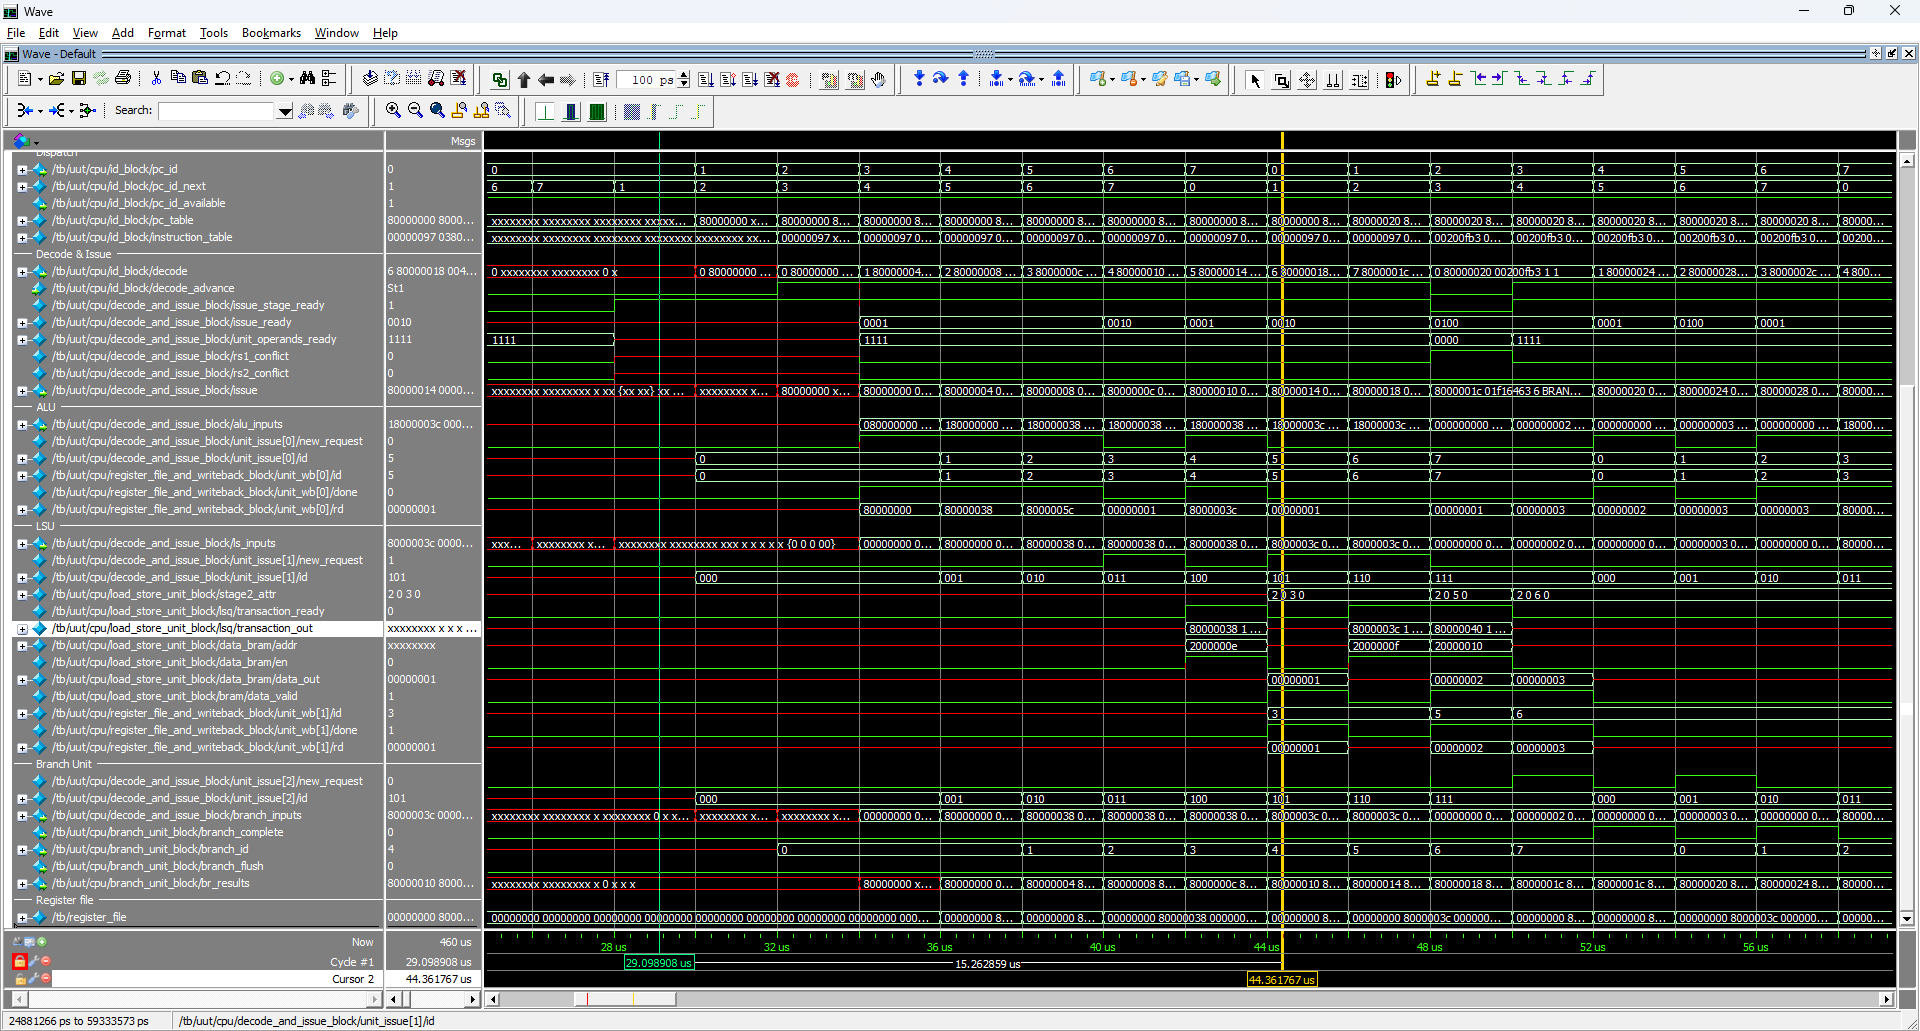
\includegraphics[width=1\linewidth]{images/05-decode.png}
    \caption{Временная диаграмма сигналов команды lw x3, 4(x1) на стадии декодирования}
    \label{fig:05-decode}
\end{figure}

\begin{figure}
    \centering
    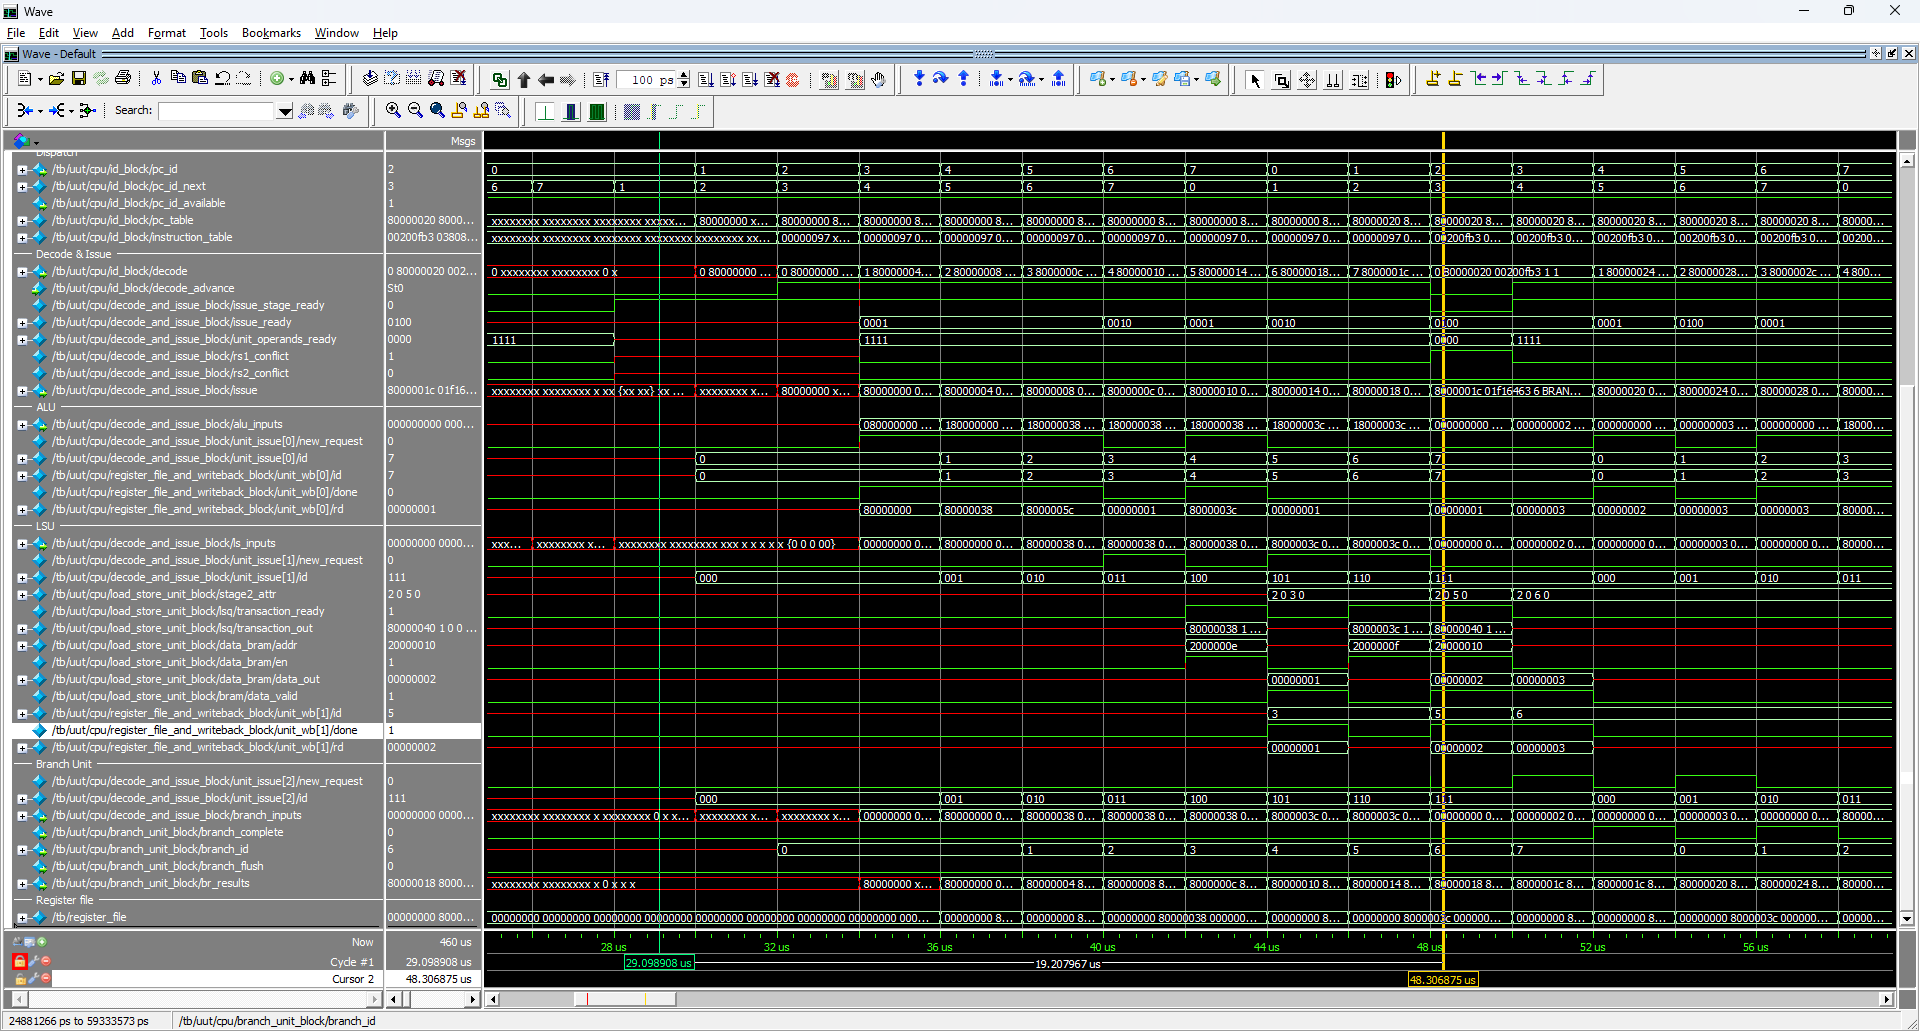
\includegraphics[width=1\linewidth]{images/05-execute.png}
    \caption{Временная диаграмма сигналов команды lw x3, 4(x1) на стадии выполнения}
    \label{fig:05-execute}
\end{figure}

Программа достаточно хорошо оптимизирована, так как планирование производилось более чем на 75\% тактах. Если же попробовать, к примеру, поменять в цикле порядок загрузки значения в регистр и ветвления, то эффективность программы снизится.

\begin{figure}
    \centering
    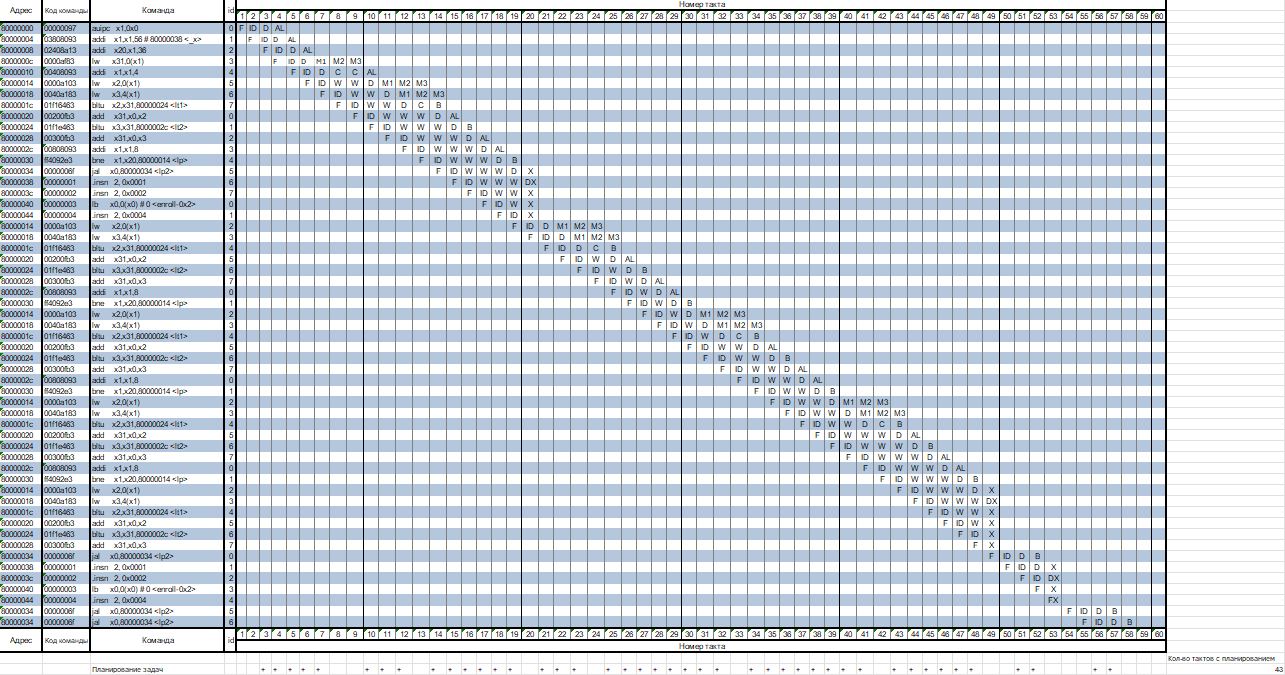
\includegraphics[width=1\linewidth]{images/05-route.png}
    \caption{Трасса работы программы}
    \label{fig:05-route}
\end{figure}